% article_EN.tex — one-page presentation of WAC for a DFIR magazine, English
% edition. The French edition is article_FR.tex, in this folder: both are
% maintained together, paragraph for paragraph.
%
% Build (LuaLaTeX, as the editor's recipe; build artefacts removed after):
%     ../build-docs.sh article_EN.tex
%
% Every figure comes from the comparison, validation and harmlessness files
% (doc/comparison, doc/validation, doc/harmlessness), measured on 9 October 2026
% on version 2.0.0. Backlog B-018.

\documentclass[10pt,a4paper,twocolumn]{article}
\usepackage[english]{babel}
\usepackage{fontspec}
\setmainfont{Noto Sans}
\setmonofont{DejaVu Sans Mono}[Scale=0.84]
\usepackage[top=13mm,bottom=13mm,left=14mm,right=14mm,columnsep=7mm]{geometry}
\usepackage{xcolor}
\usepackage{titlesec}
\usepackage{enumitem}
\usepackage{array}
\usepackage{graphicx}
\usepackage{caption}
\captionsetup{font={small,color=gris},skip=2pt}
\usepackage[hidelinks]{hyperref}
\definecolor{marine}{HTML}{0A1A33}
\definecolor{bleu}{HTML}{2F6DB5}
\definecolor{gris}{HTML}{5B6573}
\pagestyle{empty}
\setlength{\parindent}{0pt}
\setlength{\parskip}{0.35em}
\titleformat{\section}{\color{marine}\normalsize\bfseries}{}{0em}{}
\titlespacing*{\section}{0pt}{0.7em}{0.2em}
\setlist{nosep,leftmargin=1.1em}
\newcommand{\wac}{\textsc{wac}}
\newcommand{\fichier}[1]{\texttt{#1}}
\hypersetup{pdftitle={WAC — collecting Windows without leaving a trace}}

\begin{document}

\twocolumn[{%
  {\color{marine}\LARGE\bfseries WAC: collecting Windows without leaving a trace}\par
  \vspace{0.3em}
  {\color{gris}Aerospace Cyber Defence Centre of Excellence (CEC), French Air and Space Force Academy}\par
  \vspace{0.6em}
  {\itshape A collection is made on a machine that is also evidence. The tool that
  takes it must take everything, write nothing there, and be able to prove it.
  \wac{} (Windows Artefacts Collector), free software written in C++, collects
  69 artefacts of a Windows workstation by raw reading, converts them to JSON on
  the analysis workstation, and seals and logs every one of its operations. Its
  results were confronted, value by value, with those of KAPE and of Eric
  Zimmerman's tools.}\par
  \vspace{0.9em}
}]

\section{What is collected}
A single standalone executable, run from a USB key, reads the NTFS volumes raw:
the \fichier{\$MFT} and the directory indexes, without opening a file. Locked
files (hives, logs) are read like the others, and no access date changes. 69
artefacts: system and per-profile hives (the whole SAM, BAM, UserAssist,
ShimCache, Amcache, shellbags, USB), \fichier{\$MFT}, \fichier{\$UsnJrnl},
\fichier{\$LogFile}, event logs with the resources that give their text,
Prefetch, shortcuts, jump lists, SRUM, recycle bin, scheduled tasks, WMI,
persistence, Defender, browsers (history, downloads, sessions and closed tabs),
mail, DPAPI keys, the FAT and exFAT volumes of USB keys. The machine's
executables are read and their Authenticode signature checked in memory: an
authentic Microsoft binary is recorded by its fingerprints only, any other is
copied. Against KAPE (\fichier{KapeTriage}), \wac{} takes everything KAPE
takes --- 5 \fichier{desktop.ini} aside --- and 790 more files, in 41~s
against 44.

\section{A procedure kept}
\wac{} \emph{collects} on the examined machine or \emph{converts} on the
analysis workstation, never both. Every exhibit enters a sealed
\textbf{exhibit store}: its manifest gives, for each, MD5, SHA-1 and SHA-256,
the original's eight NTFS dates (\fichier{\$STANDARD\_INFORMATION} and
\fichier{\$FILE\_NAME}), its MFT entry and the reading method; the manifest's
fingerprint seals it. After the initial copy, the store is neither read nor
written again: the conversion first checks the seal and every fingerprint,
refuses a retouched exhibit, then works on a working copy, where the logs of the
hives and ESE databases are replayed. Every operation is written to the
\textbf{investigation log} (\fichier{investigation.json}): instant, target,
result, the trace it is expected to leave, and the time of each step. Two
shipped scripts recheck a store without \wac{}.

\section{JSON, not CSV}
One file per artefact, typed values (numbers, booleans, nested lists), every
date to 100\,ns in UTC and in the suspect's local time, with the offset in force
\emph{at that date}. A field without a value is not emitted: no zero, no 1601
date that would read as data. Each event's text is rendered as Windows displays
it. The result loads as is into an analysis tool.

\section{No trace, measured}
On a frozen clone of the test machine, each tool is run from a key, under
Sysmon, the NTFS change journal bounded before and after. \wac{} writes
\textbf{no file} on C:, \textbf{no registry value}, no event in Windows' logs;
it starts no process and sends nothing on the network. What remains are the
Amcache entry and the ShimCache entry Windows creates for any program, and what
a monitoring records of its execution (Sysmon: the process, two raw reads of a
volume). Under the same conditions, KAPE writes to the user's hive, and its
modules 28 files on C:. The build script refuses a \fichier{WAC.exe} that would
import a function able to start a process.

\section{Tests that can fail}
An autonomous cycle, in a Windows~11 virtual machine, lays witnesses of known
value (files, registry, browsers, mail, a 261-character path), collects,
converts, and passes 494 checks. Each confronts \wac{} with an independent
source: Windows itself (\fichier{Get-WinEvent}, \fichier{Get-FileHash},
registry), \fichier{dissect.esedb}, Python's SQLite and \fichier{lz4}. A second
conversion must give the same JSON files, byte for byte. Against Eric
Zimmerman's eleven tools, on the same exhibits, each difference was settled by
such a source: \wac{}'s values are the same, or more accurate (RECmd rolls hives
back to an older state, AmcacheParser invents 3,450 values, EvtxECmd is wrong on
ten).

\section{In figures}
\begin{tabular}{@{}>{\raggedright\arraybackslash}p{0.8\columnwidth}@{\hspace{0.5em}}r@{}}
Artefacts collected & 69 \\
Collection without the executables (KAPE: 44~s) & 41~s \\
Whole conversion, store checked & 80~s \\
Files written on C: by \wac{} & 0 \\
Checks of the test cycle & 494 \\
Reference tools confronted & 12 \\
\end{tabular}

\section{Availability}
Version 2.0.0, Windows~10 and 11 (x64), GPL~3.0 licence:
\url{https://github.com/dev-cec/WAC}. Manuals, validation, harmlessness and
comparison files in English and French.


\vfill
\begin{center}
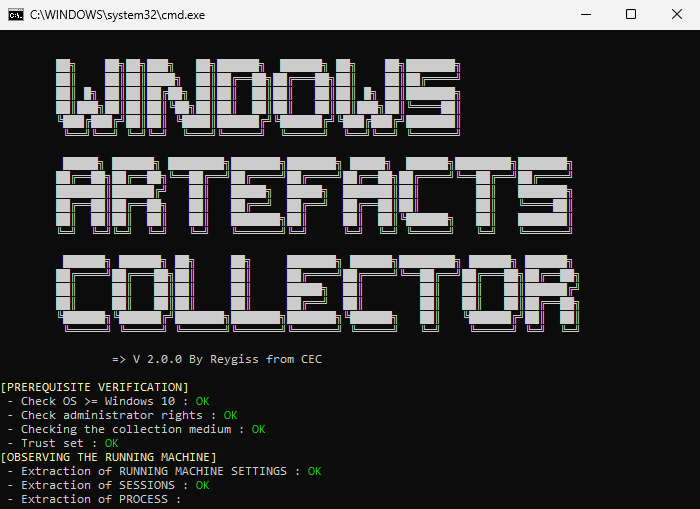
\includegraphics[width=\columnwidth,height=46mm,keepaspectratio]{../images/wac-running_EN.png}
\captionof*{figure}{\wac{} collecting.}
\end{center}

\end{document}
